\documentclass[letterpaper,12pt]{article}
\usepackage[utf8]{inputenc}
\usepackage{amsmath}
\usepackage{amsfonts}
\usepackage{amssymb}
\usepackage{enumerate}
\usepackage[margin=0.75 in]{geometry}
\usepackage{graphicx}
\usepackage{hyperref}

\newcommand{\aaa}{\mathbf{a}}
\newcommand{\bbb}{\mathbf{b}}
\newcommand{\abs}[1]{\lvert #1\rvert}
\newcommand{\len}[1]{\lVert #1\rVert}
\newcommand{\dotp}{\boldsymbol{\cdot}}
\renewcommand{\r}{\mathbf{r}}
\newcommand{\x}{\mathbf{x}}
\newcommand{\R}{\mathbb{R}}
\newcommand{\di}{\displaystyle}
%opening
\title{A triple integral example}
\author{Sean Fitzpatrick}

\begin{document}

\maketitle

Since my first example from today's class was mostly effective in demonstrating the difficulty of setting up a triple integral, and less so on how to actually get it done, here it is again: we wish to evaluate the integral 
\[
\iiint_E z\,dV,
\]
where $E$ is the region in the first octant bounded by the cylinder $y^2+z^2=9$ and the planes $x=0$, $y=3x$, and $z=0$. The sketch of the region is as follows:
\begin{center}
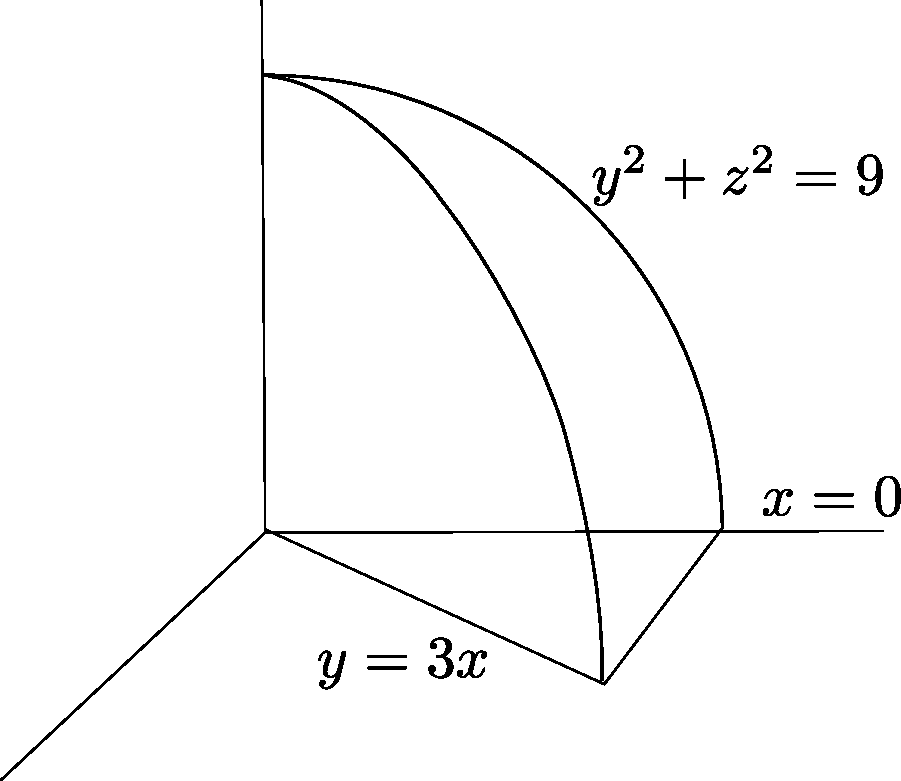
\includegraphics[width=4in]{triple_eg.pdf}
\end{center}
Note that the region of integration projects to a region in the $xy$-plane bounded by $x=0$ and $y=3x$. To close off this region, we note that since we must have $y^2+z^2\leq 9$, it follows that $y\leq 3$, so we have the triangle bounded by $x=0$, $y=3x$, and $y=3$. The region of integration then lies between the plane $z=0$ and the cylinder $z=\sqrt{9-y^2}$, and above our triangle in the $xy$-plane, which is given by the inequalities $0\leq x\leq 1$ and $3x\leq y\leq 3$. The iterated integral is therefore
\begin{align*}
\iiint_E z\,dV &= \int_0^1\int_0^{3x}\int_0^{\sqrt{9-y^2}}z\,dz\,dy\,dx\\
& = \int_0^1\int_{3x}^3\frac{1}{2}(9-y^2)\,dy\,dz\\
& = \int_0^1\frac{1}{2}\left[9y-\frac{1}{3}y^3\right]_{3x}^3\,dx\\
& = \int_0^1\left(\frac{27}{2}-\frac{9}{2}-\frac{27}{2}x+\frac{9}{2}x^3\right)\,dx\\
& = \left.\frac{9}{8}x^4-\frac{27}{4}x^2+\frac{18}{2}x\right|_0^1\\
& = 27/4.
\end{align*}
If we wanted to treat our triangle as a Type II region, given by $0\leq y\leq 3$ and $0\leq x\leq y/3$, we would instead have
\[
\iiint_E z\,dV = \int_0^3\int_0^{y/3}\int_0^{\sqrt{9-y^2}}z\,dz\,dx\,dy,
\]
and you can check that the result is the same. The other orders of integration are less natural, but still possible. If we wanted to integrate first with respect to $x$, we would note that $0\leq x\leq y/3$, with $y^2+z^2\leq 9$ giving our region of integration in the $yz$-plane. If we wrote this region as $0\leq y\leq \sqrt{9-z^2}$ with $0\leq z\leq 3$, we would have the integral
\[
\iiint_E z\,dV = \int_0^3\int_0^{\sqrt{9-z^2}}\int_0^{y/3}z\,dx\,dy\,dz,
\]
with a similar integral if we reversed the order of $y$ and $z$. Finally, if we wanted to integrate first with respect to $y$, we would have to note that for a given $x$ and $z$, $y$ runs from $y=3x$ to $y=\sqrt{9-z^2}$. To determine the region of integration in the $xz$-plane, we note that when the cylinder $y^2+z^2=9$ intersects the line $y=3x$, we have $(3x)^2+z^2=9$, or $9x^2+z^2=9$. Our region is thus bounded by $x=0$, $z=0$ and the ellipse $9x^2+z^2=9$. If we write this as $0\leq x\leq 1$ with $0\leq z\leq 3\sqrt{1-x^2}$, then we have
\[
\iiint_Ez\,dV = \int_0^1\int_0^{3\sqrt{1-x^2}}\int_{3x}^{\sqrt{9-z^2}}z\,dy\,dz\,dx,
\]
with a similar integral for the order $dy\,dx\,dz$.




\end{document}
